\documentclass[tikz, border=12pt]{standalone}
\usepackage{amsmath}
\usetikzlibrary{positioning, arrows.meta}
\begin{document}
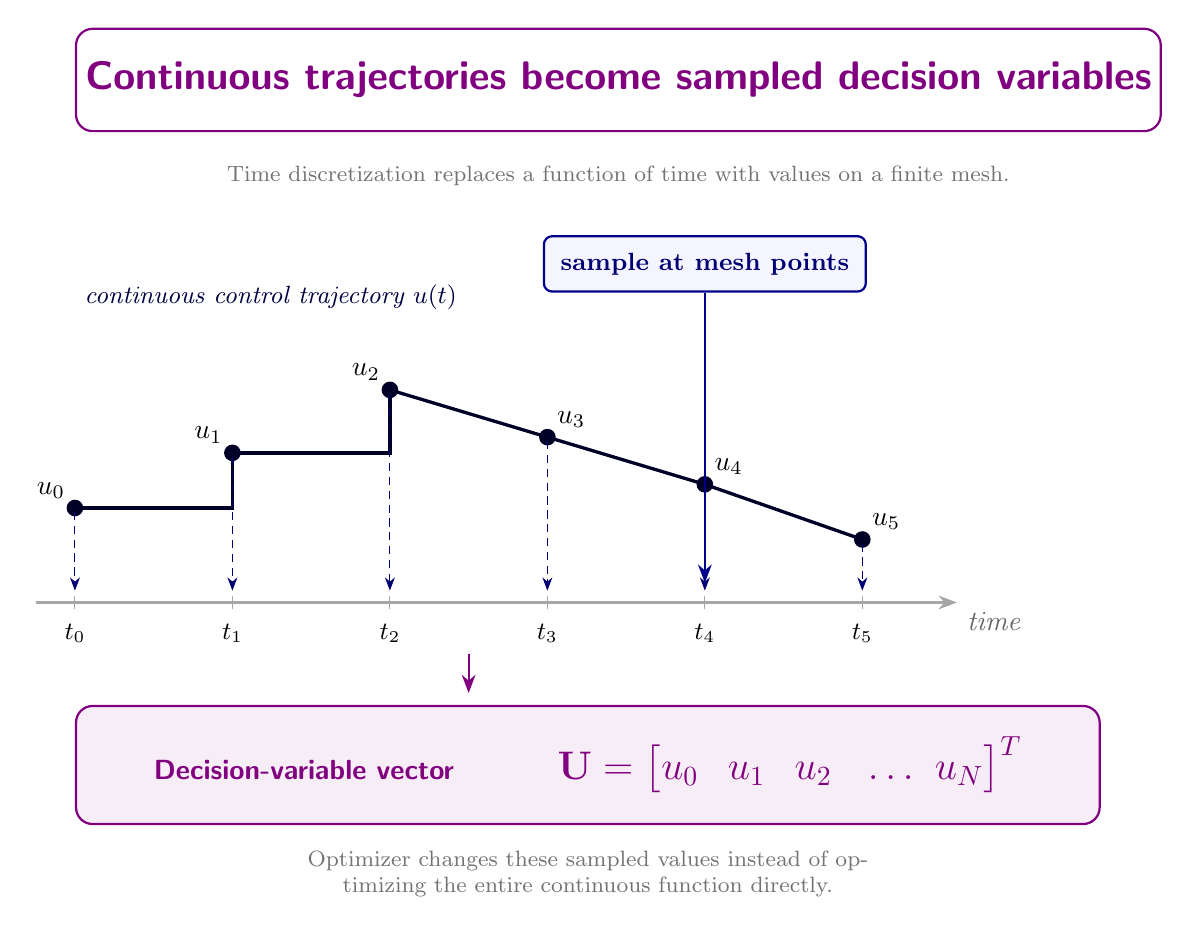
\begin{tikzpicture}[
    font=\sffamily,
    >=Stealth,
]

% ---- Title box ----
\node[draw=violet, thick, rounded corners=6pt, minimum width=13cm, minimum height=1.3cm,
      align=center, anchor=north west] (titlebox) at (0,0)
    {\textcolor{violet}{\bfseries\Large Continuous trajectories become sampled decision variables}};

\node[below=3mm of titlebox.south, font=\footnotesize, text=black!55]
    {Time discretization replaces a function of time with values on a finite mesh.};

% ---- Plot region ----
\begin{scope}[shift={(0,-7.3)}]

    \node[font=\itshape\small, text=blue!25!black, anchor=south west] at (0,3.6)
        {continuous control trajectory $u(t)$};

    % t-positions and u-heights
    % t0=0 t1=2 t2=4 t3=6 t4=8 t5=10
    % u0=1.2 u1=1.9 u2=2.7 u3=2.1 u4=1.5 u5=0.8

    % step part: u0 -> u1 -> u2 (zero-order hold)
    \draw[very thick, blue!15!black]
        (0,1.2) -- (2,1.2) -- (2,1.9) -- (4,1.9) -- (4,2.7);
    % declining straight-line part: u2 -> u3 -> u4 -> u5
    \draw[very thick, blue!15!black]
        (4,2.7) -- (6,2.1) -- (8,1.5) -- (10,0.8);

    % sample points
    \foreach \x/\y in {0/1.2, 2/1.9, 4/2.7, 6/2.1, 8/1.5, 10/0.8}
        \fill[blue!15!black] (\x,\y) circle (3pt);

    % point labels
    \node[above left, font=\itshape] at (0,1.2)  {$u_0$};
    \node[above left, font=\itshape] at (2,1.9)  {$u_1$};
    \node[above left, font=\itshape] at (4,2.7)  {$u_2$};
    \node[above right, font=\itshape] at (6,2.1) {$u_3$};
    \node[above right, font=\itshape] at (8,1.5) {$u_4$};
    \node[above right, font=\itshape] at (10,0.8){$u_5$};

    % dashed drop-lines from each point to the axis
    \foreach \x/\y in {0/1.2, 2/1.9, 4/2.7, 6/2.1, 8/1.5, 10/0.8}
        \draw[densely dashed, ->, blue!45!black] (\x,{\y-0.05}) -- (\x,0.15);

    % time axis
    \draw[->, thick, gray!70] (-0.5,0) -- (11.2,0) node[below right, font=\itshape, text=black!60] {time};
    \foreach \x in {0,2,4,6,8,10}
        \draw[gray!70] (\x,-0.08) -- (\x,0.08);
    \node[below, font=\small] at (0,-0.15)  {$t_0$};
    \node[below, font=\small] at (2,-0.15)  {$t_1$};
    \node[below, font=\small] at (4,-0.15)  {$t_2$};
    \node[below, font=\small] at (6,-0.15)  {$t_3$};
    \node[below, font=\small] at (8,-0.15)  {$t_4$};
    \node[below, font=\small] at (10,-0.15) {$t_5$};

    % "sample at mesh points" callout, pointing down to t4
    \node[draw=blue!55!black, thick, rounded corners=3pt, fill=blue!4,
          font=\bfseries\small, text=blue!45!black, inner sep=6pt] (callout) at (8,4.3)
        {sample at mesh points};
    \draw[->, thick, blue!55!black] (callout.south) -- (8,0.25);

\end{scope}

% ---- Decision-variable vector box ----
\draw[->, thick, violet] (5,-7.95) -- (5,-8.45);

\node[draw=violet, thick, rounded corners=6pt, fill=violet!7,
      minimum width=13cm, minimum height=1.5cm, anchor=north west, inner sep=10pt]
      (vecbox) at (0,-8.6)
    {\textcolor{violet}{\bfseries Decision-variable vector}\hspace{1.2cm}
     \textcolor{violet}{\bfseries\Large $\mathbf{U} = \big[u_0\ \ u_1\ \ u_2\ \ \ldots\ u_N\big]^{T}$}};

\node[below=2mm of vecbox.south, font=\footnotesize, text=black!55, align=center,
      text width=13cm]
    {Optimizer changes these sampled values instead of optimizing the entire continuous function directly.};

\end{tikzpicture}
\end{document}
